% !TEX program = xelatex
\documentclass[UTF8,11pt,a4paper]{ctexart}
\usepackage[a4paper,margin=2.2cm]{geometry}
\usepackage{amsmath,bm,booktabs,graphicx,float,tabularx,hyperref}
\hypersetup{colorlinks=true,linkcolor=blue,urlcolor=blue,pdftitle={APMCM B题问题4：偏好变化与鲁棒推荐}}
\title{问题4：偏好变化与偏好鲁棒设计}
\author{}\date{}
\begin{document}\maketitle

\section{问题目标}
问题3给出了三目标Pareto前沿，但实际决策者对热阻$R$、压降$P$和温度非均匀性$U$的重视程度可能不同。本问研究权重变化如何改变推荐结构，并寻找在给定偏好集合内最小化最坏机会损失的方案。

\section{偏好模型}
沿用问题3的理想点$\bm F^{\rm I}$和Nadir点$\bm F^{\rm N}$，定义
\[
z_k(x)=\frac{F_k(x)-F_k^{\rm I}}{F_k^{\rm N}-F_k^{\rm I}},\qquad
G(x;w)=\max_k\{3w_kz_k(x)\}+10^{-4}\sum_k3w_kz_k(x),
\]
其中$w_k\ge0$且$\sum_kw_k=1$。增强切比雪夫主项控制最差标准化退让，小增强项只用于打破并列。对每个权重，定义专属最优评分
\[
G^*(w)=\min_{x\in\mathcal P_{ref}}G(x;w),
\]
以及绝对机会损失$r_a(x,w)=G(x;w)-G^*(w)$。同时使用相对机会损失
\[
r_r(x,w)=\frac{G(x;w)-G^*(w)}{G^*(w)}
\]
检验结论对遗憾定义的敏感性。

\section{权重域与求解}
考察三类偏好域：完整权重单纯形、$w_k\ge0.1$的平衡偏好域，以及$w_R\ge0.5$的散热优先域。完整单纯形采用$H=50$离散，含1326组权重，并以$H=25,100$检查收敛。对每个权重先在问题3合并Pareto集上搜索，再对候选连续精化。偏好鲁棒解定义为
\[
x^{rob}=\arg\min_x\max_{w\in\mathcal W}r(x,w).
\]

\section{结果}
\begin{table}[H]\centering\small
\caption{权重域和遗憾定义下的推荐方案}
\begin{tabular}{llrrrr}\toprule
权重域&遗憾定义&$a$&$b$&$N$&最大遗憾\\\midrule
完整单纯形&绝对&0.224932&4.5000&6&1.158963\\
完整单纯形&相对&0.224932&4.5000&6&0.386426\\
$w_k\ge0.1$&绝对&0.217000&3.4500&4&0.801105\\
$w_k\ge0.1$&相对&0.224932&4.5000&6&0.352589\\
$w_R\ge0.5$&绝对&0.233500&3.3675&8&0.669244\\
$w_R\ge0.5$&相对&0.225500&3.1913&4&0.316329\\\bottomrule
\end{tabular}
\end{table}
不同遗憾定义具有不同数值尺度，最大遗憾只能在同一定义内比较。完整单纯形下，绝对和相对遗憾均选择$N=6$；偏好域收缩后，推荐可切换到$N=4$或$N=8$，说明不存在脱离偏好域的唯一最优结构。

\begin{figure}[H]\centering
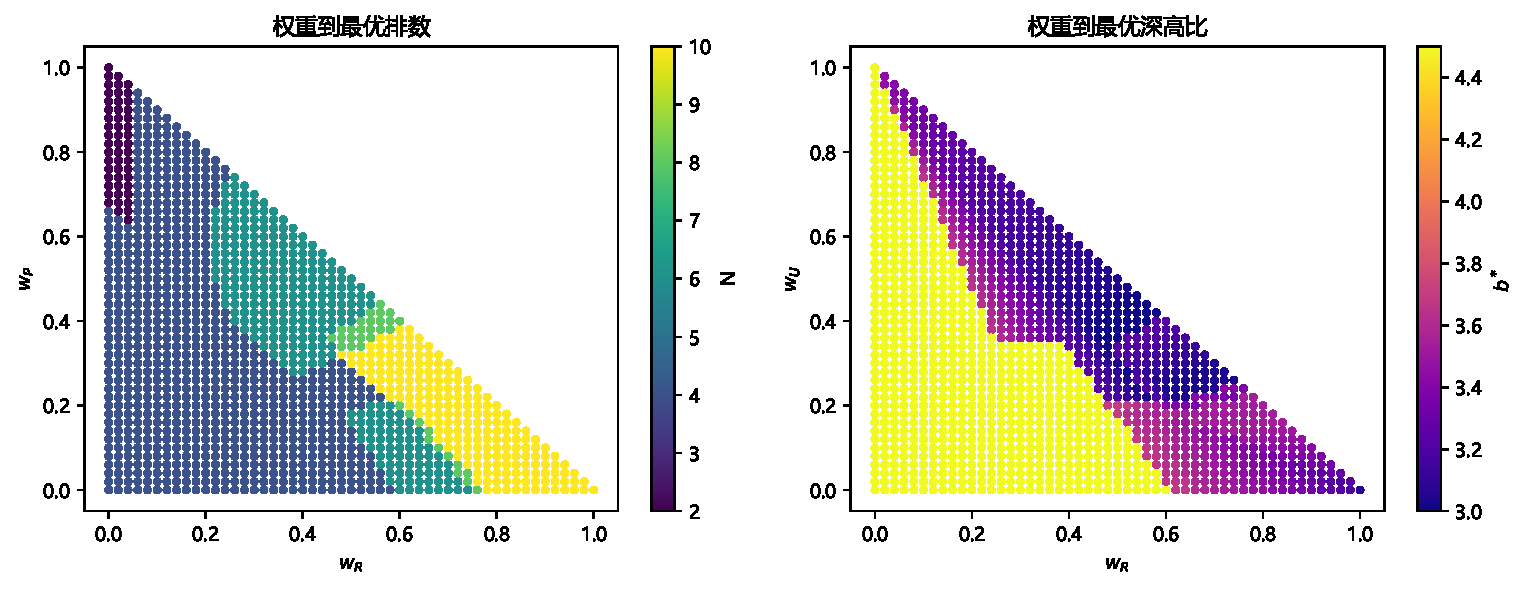
\includegraphics[width=.90\linewidth]{../figures/fig_q4_01_weight_mapping.pdf}
\caption{完整权重单纯形上最优结构的分布}
\end{figure}

在完整单纯形中，$N=2,4,6,8,10$的获胜权重区域占比分别约为3.85\%、55.81\%、22.70\%、2.64\%和15.01\%。$N=4$覆盖的偏好区域最多，而$N=6$最小化最坏机会损失；二者回答的问题不同，并不矛盾。$H=25,50,100$均得到同一完整单纯形最小最大遗憾方案，表明该离散精度下推荐稳定。

\section{问题4结论}
当不给出额外偏好且允许完整权重单纯形时，推荐
\[
\boxed{(a,b,N)=(0.224932,4.5000,6)}.
\]
该结论的含义是完整偏好域内的最坏机会损失最小，而不是在所有可能偏好定义下唯一最优。若决策者限制权重范围，必须重新使用相应权重域和遗憾定义选择结构。
\end{document}

